\documentclass{article}
\usepackage{amsmath, graphicx, natbib, tikz}
\usepackage[margin=1in]{geometry}

\setlength{\parindent}{0pt}

\title{Problem Set 1}
\author{Ayse Mehmeti}
\date{Fall 2025}

\begin{document}
\maketitle

\section*{Research Interest}

My research project explores whether the opening of vape shops near public schools in Florida leads to an increase in vaping-related disciplinary actions among students. Many studies have already shown that when vape shops are located close to where teenagers live or go to school, they are more likely to try or regularly use vaping products. However, it is not well studied whether this increased access to vape products also leads to more students getting caught and punished for vaping at school. This project will fill that gap by focusing on actual school discipline records rather than self-reported vaping behavior.

Prior research has shown that vape shops are disproportionately located in minority communities and near schools, raising concerns about health equity \citep{venugopal2020vape}. Other studies have found that the presence of e-cigarette retailers near schools increases the likelihood of experimentation among middle school students \citep{bostean2016ecig}. These findings motivate my project to test whether school discipline records show evidence of increased vaping violations after vape shops open nearby.

I will use a panel dataset that covers the years 2021 to 2024. It includes yearly data on how many students in each school were disciplined for vaping, as well as address information for all public schools in Florida. I also have access to a list of tobacco-licensed shops in Florida, which includes the names, locations, and effective license dates of vape sellers. By calculating the distance between schools and vape shops, I will be able to identify which schools had a vape shop open within 1,000 feet after 2021. These schools will be considered ``treated.'' Schools that never had a vape shop nearby between 2021 and 2024 will be used as the control group.

I will apply a Difference-in-Differences method to compare the trends in vaping-related discipline before and after vape shops opened near treated schools, relative to schools that had no vape shop nearby. One difficulty with this project is that I only have data starting in 2021, so I cannot observe long-term trends before that. To address this, I will focus on schools where the vape shop opened in 2022 or later and use 2021 as the comparison year.

Another challenge is that not all tobacco license holders actually sell vape products, so I will filter the shop list by name and type, keeping only vape and smoke shops, gas stations, and convenience stores, and leaving out places like bars, restaurants, and wholesalers. I will also run extra tests using only dedicated vape shops to check whether the results are stronger or weaker depending on the type of store.

Differences in school discipline policies could also affect the data. I will include school fixed effects by adding school details that can affect discipline. I have data on each school’s Title I status, student performance, and school type. Controlling for these will help me see if vape shop openings are the real cause of more disciplinary actions, and not other differences between schools. I will also include year fixed effects to control for statewide changes, such as new policies like adding vape detectors at certain schools.

This study aims to provide clear evidence on whether vape shop exposure increases the chance of students being disciplined for vaping. The idea is that more exposure to vape shops may lead to more student use, which may then lead to more students being caught and punished. The results can help guide future decisions on zoning laws, retail regulations, and school safety strategies.

\section*{Equation Example}
To illustrate, I include a common econometric model framework:
\[
Y_{it} = \alpha + \beta \text{Treated}_{it} \times \text{Post}_{t} + \gamma X_{it} + \mu_i + \lambda_t + \epsilon_{it}
\]

\begin{figure}[h]
\centering
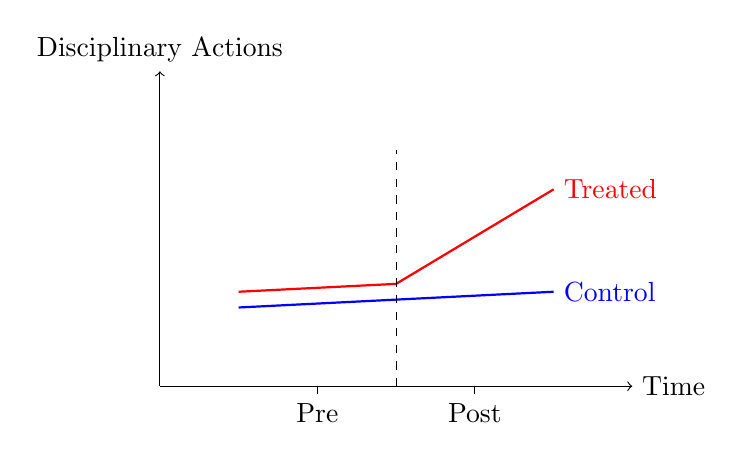
\begin{tikzpicture}[scale=1.0]

% Axes
\draw[->] (0,0) -- (6,0) node[right]{Time};
\draw[->] (0,0) -- (0,4) node[above]{Disciplinary Actions};

% Labels for time periods
\draw (2,0) -- (2,-0.1) node[below]{Pre};
\draw (4,0) -- (4,-0.1) node[below]{Post};

% Control group line (flat)
\draw[thick, blue] (1,1) -- (5,1.2) node[right]{Control};

% Treated group line (increase after post)
\draw[thick, red] (1,1.2) -- (3,1.3) -- (5,2.5) node[right]{Treated};

% Dotted vertical line at intervention
\draw[dashed] (3,0) -- (3,3);

\end{tikzpicture}
\caption{Illustrative Difference-in-Differences (DiD) figure: treated vs. control schools before and after vape shop openings.}
\end{figure}

\bibliographystyle{apalike}
\bibliography{references}

\end{document}
